\documentclass[11pt,reqno]{article}
\newcommand{\vet}[1]{{\ensuremath{\mbox{\boldmath $#1$}}}}
\renewcommand{\baselinestretch}{1.5}
\setlength{\oddsidemargin}{0in} \setlength{\textwidth}{6in}
\setlength{\topmargin}{-0.2in} \setlength{\textheight}{8.8in}
\def\labelitemi{--}
\usepackage{graphicx}
\usepackage{amsmath}
\usepackage[T1]{fontenc}
\usepackage{lmodern}
\usepackage{amssymb,amsmath}
\usepackage{natbib}
\usepackage[linkcolor=blue]{hyperref}
\usepackage[title]{appendix}
%\usepackage{xurl}
\usepackage{booktabs}
% \addbibresource{bes.bib}

% xelatex bes_intro_paper
% bibtex  bes_intro_paper
% xelatex bes_intro_paper
% xelatex bes_intro_paper




\begin{document}

\titlepage
\title{\textbf{Bayesian Evidence Synthesis for Informative Hypotheses: An introduction}}
\author{\textbf{Irene Klugkist, Thom Benjamin Volker} \\
Methodology and Statistics, Social and Behavioral Sciences, Utrecht University} \maketitle



\noindent \textbf{Abstract}

\noindent To establish a theory one needs cleverly designed and well executed studies with appropriate and correctly interpreted statistical analyses. Equally important, one also needs replications of such studies and a way to combine the results of several replications into an accumulated state of knowledge. An approach that provides an appropriate and powerful analysis for studies targeting pre-specified theories is the use of Bayesian informative hypothesis testing. An additional advantage of the use of this Bayesian approach is that combining the results from multiple studies is straightforward. In this paper we discuss the behavior of Bayes factors in the context of evaluating informative hypotheses with multiple studies. By using simple models and (partly) analytical solutions we introduce and evaluate Bayesian Evidence Synthesis (BES) and compare its results to Bayesian Sequential Updating (BSU). By doing so we clarify how different replication or updating questions can be evaluated. In addition, we illustrate BES with two simulations, in which multiple studies are generated to resemble conceptual replications. The studies in these simulations are too heterogeneous to be aggregated with conventional research synthesis methods.


\bigskip

\noindent Keywords and phrases: Bayesian evidence synthesis, Bayes factors, Bayesian updating, Informative hypotheses, Replication


\newpage

\section{Introduction}
\label{intro}


For any empirical science, replicability is an essential topic. There are several papers on the need for replication, including explanations on reasons for lack of replication studies and recommendations on how to increase replicability \citep{asendorpf_replication_2013, simonsohn_telescopes_2015, verhagen_bayesian_2014, nosek_replicability_review_2021}.
Especially, the replication crisis in psychology (and other fields) initiated several initiatives in this area, for instance, the Reproducibility Project \citep{open_science_collab_2015, open_science_collab_2012} and the Registered Replication Reports initiative \citep{simons_registered_2014}. Also, several journals are devoted to, or reserve specific sections of their journal for reports of replication studies (e.g., Royal Society Open Science, Journal of Personality and Social Psychology, Archives of Scientific Psychology, Journal of Experimental Psychology: General).

It is important to distinguish between different types of replication studies, based on how similar the studies are in their design. \textit{Direct}, \textit{close} or \textit{exact replications} aim for as much similarity with the original study as possible, such that the only difference is that in the replication study new data has been collected \citep{simons_direct_2014, brandt_et_al_replication_2014}. Aggregation of results from exact replications is relatively straightforward. If a study is a strictly exact replication of the initial study and the raw data from both studies are available, then the data can be combined and analyzed as if it was one large study. In practice, usually other approaches are used, for instance, within the Bayesian framework, one could apply Bayesian Sequential Updating \citep[BSU;][]{schonbrodt_sequential_2017}. This provides a summary of results after the initial study, an updated summary after adding one replication, a further updated summary after adding another replication, and so forth. The final result of Bayesian updating of data from multiple studies is exactly the same as the result of one Bayesian analysis of all data combined, as long as the same initial prior is used.

Another common approach to aggregation of multiple studies is (Bayesian) meta-analysis \citep[see][]{lipsey_wilson_2001, sutton_bayesian_meta2001}. One advantage of the meta-analysis approach is that one does not need the raw data of the studies. The aggregation is at the level of summary statistics (e.g., effect sizes and standard errors) which are often available in the publications of the separate studies. Another difference making meta-analysis more flexible is that studies do not have to be strictly exact replications. With random effects meta-analysis and the option of adding moderators to explain differences between studies, the model accounts for and potentially helps understanding heterogeneity in the results. Still, aggregating results using meta-analysis requires a relatively high level of similarity between studies. Since the aggregation is at the level of effect sizes, comparable effect sizes must be available for all studies to be synthesized. For studies that are theoretically related but methodologically highly diverse meta-analyzing the results may not be feasible.

In the context of \textit{indirect} or \textit{conceptual replications} the studies may indeed be highly diverse. One common theory may be investigated in different contexts, with different study designs, using different instruments, variables, and statistical analyses. An advantage of performing conceptual replications is that results that agree across different methodologies and contexts jointly provide stronger support for the underlying central theory \citep{crandall_conceptual_2016, lawlor_triangulation_2017, nosek_scientific_2012}. A disadvantage is that the aggregation of results of conceptual replications is not straightforward.

\citet{kuiper_combining_2013} proposed a method based on combining evidence for informative hypotheses on the level of Bayes factors. The underlying idea is that the central theory of interest is allowed to be operationalized differently in each study. The study specific informative hypothesis, that represents the central theory, is evaluated using the Bayes factor, which measures the support in the data for the hypothesis of interest against some alternative. Stated differently, the Bayes factor quantifies, based on the observed data, the change from the prior odds of two competing hypotheses to the posterior odds of those hypotheses. Aggregation of evidence from multiple studies is done by using the posterior odds after the first data set as the prior odds for the next (i.e., a replication study). This provides updated (with each new replication) relative support measures for the two hypotheses that are compared.

Using this approach, each study provides a level of evidence for the central theory despite the diversity in study design. Although it has been applied successfully \citep{zondervan_parental_2019, zondervan_robust_2020, kevenaar_bes_2021, volker_cooperation_2022}, a paper describing the correct interpretation of the combined evidence and the advantages and limitations of this approach is currently lacking. The main goal of this article is therefore to provide a clear and correct understanding of this Bayesian Evidence Synthesis (BES) approach, that is based on combining Bayes factors that result from evaluating informative hypotheses.

In the next section, we demonstrate the behavior of Bayes factors for an inequality constrained hypothesis in one study. The use of Bayesian informative hypothesis testing is shortly outlined and the Bayes factor is introduced using a simple binomial example. Subsequently, we consider the synthesis of results from multiple studies. The starting point is an example where a set of exact replications is available, again using the binomial model as illustration, and comparing results of BES and BSU. This is followed by an example in the context of conceptual replications, where BES is applied to a set of highly diverse studies in simulations. The paper ends with a discussion of results and recommendations for potential users of BES, as well as for future methodological research. All materials to reproduce these examples can be found on GitHub \citep[][https://github.com/thomvolker/bes-intro-paper]{klugkist_bes_materials}.




\section{Bayes factors for informative hypotheses in one study}
\label{theory}

Informative hypotheses are defined as hypotheses that impose constraints on model parameters, or functions of parameters, to reflect specific expectations of researchers \citep{hoijtink_informative_2012}. One example is a hypothesis imposing order constraints on the parameters of interest, for example, on subgroup means in analysis of variance, or on a set of regression coefficients in multiple regression models. In addition, informative hypotheses can be specified using equality constraints, about equality constraints and range restrictions and the constraints can be on combinations or functions of parameters (e.g. on differences between means or odds ratios). There are several papers motivating why informative hypothesis testing is a valuable alternative to null hypothesis significance testing \citep[NHST;][]{beland2012informative, vanrossum_hypothesis_2013, klugkist_confirmatory_2014, regenwetter_cavagnaro_2019} and there are many applications of informative hypothesis evaluation in psychology, for instance, see: \citet{cooper_relationship_2014, bullens_role_2011, vanuijlen_approach_behavior_2017, flore_influence_2018, matthijssen_effects_2019}.
Note that informative hypotheses can be evaluated in the frequentist framework \citep[e.g.,][]{silvapulle_sen_2004, kuiper_goric_2011, altinisik_gorica_2021}, but we only consider Bayesian informative hypotheses testing based on the Bayes factor.

There are many references that explain the Bayes factor in general \citep{kass_raftery_bayes_factors_1995, hoijtink_tutorial_2019, heck_review_2022} as well as in the specific context of testing informative hypotheses \citep[e.g.,][]{klugkist_inequality_2005, gu_inequality_2014, hoijtink_informative_2012}. The Bayes factor compares two models or hypotheses $H_1$ and $H_2$, by:
\begin{equation*}
  BF_{1,2} = \frac{P(D|H_1)}{P(D|H_2)},
\end{equation*}

\noindent where $P(D|H_1)$ and $P(D|H_2)$ are the marginal likelihoods denoting the probability that the data was generated under $H_1$ versus the probability that the data was generated under $H_2$. So, when the resulting value is larger than one, there is more support for $H_1$, whereas $BF_{1,2}<1$ implies more support for $H_2$.

The evaluation of an informative hypothesis using Bayes factors therefore always requires the formulation of at least one alternative hypothesis. We discuss three natural choices: the unconstrained alternative, the complement of the informative hypothesis and the null hypothesis. Although Bayes factor testing against each of these alternatives is not new, an explicit comparison between the different alternatives has not been made and serves two purposes. It provides guidelines for future users, who often find it difficult to make such choices and it provides information that is relevant for the next step: aggregating Bayes factors over studies.

In the next subsections, we shortly outline the choice of competing hypotheses and the estimation of BFs as implemented in the \texttt{R}-package \texttt{BFpack} \citep{BFpack}. The numerical comparison of results for the three different alternative hypotheses is, however, done using a simple binomial example using analytical solutions for the Bayes factors of interest. The conclusions we can draw from the binomial example, however, also extend to other examples and statistical models.




\subsection{Testing against the different alternatives}

From here, let the interest be to evaluate if and to what extent the data support a simple ordering of parameters (hypothesis $H_i$). In the context of an experimental design with 3 conditions, the informative hypothesis stating that the mean score on the outcome of interest (denoted $\mu$) increases from condition 1 to 2 to 3 could be an explicit expectation from the researcher designing this experiment. In order to evaluate this expectation ($H_i: \mu_1 < \mu_2 < \mu_3$), the researcher needs to decide on one or more competing hypotheses.

One option is to use the unconstrained hypothesis. Similar to the alternative hypothesis in NHST, this hypothesis does not impose any constraints and as such does not reflect a theory or specific expectation. Comparing an informative hypothesis against the unconstrained alternative is a way to test the support for the constraints imposed by the informative hypothesis. Another option is to test $H_i$ against its complement (denoted $H_c$), that is, the collection of all orderings that is not $H_i$. This also provides the level of support for the informative hypothesis of interest \citep[see][]{hoijtink_informative_2012, vandeun_testing_2009, vanrossum_hypothesis_2013}. The main difference between the two alternatives is that $H_i$ is nested in the unconstrained hypothesis, while $H_i$ and $H_c$ describe mutually exclusive parts of the parameter space. This has an effect on the (maximum) level of support in the resulting Bayes factors, as we will see and further discuss in the binomial example. A third option is testing the informative hypothesis against the null hypothesis. Although the null hypothesis has been criticized as a potentially unrealistic option \citep[e.g.,][]{cohen_earth_1994, krueger_null_2001, lykken_wrong_1991} and usually does not represent a theoretical expectation of the researcher, it is still a popular alternative. Often, researchers prefer to include and evaluate the option that there is no effect in the population and thus all sample effects are likely to be chance results. Therefore, they may want to compare the theoretical expectation with the hypothesis stating that there are no effects at all.


The computation of Bayes factors for informative hypotheses was first proposed by \citet{klugkist_inequality_2005} and based on testing an informative hypothesis against the unconstrained alternative $H_u$, with what was called the encompassing prior approach \citep[see also][]{hoijtink_klugkist_boelen_2008, hoijtink_informative_2012}. In a nutshell the idea is as follows. Any informative hypothesis can be seen as the unconstrained hypothesis plus a set of constraints. The encompassing prior approach uses this property by deriving an expression for the Bayes factor, $BF_{i,u}$, that requires only evaluation of the unconstrained model and determining the volume of the region that is in agreement with the constraints. Such evaluation of the posterior distribution of the parameters provides a measure of fit for the constrained model relative to the unconstrained model (denoted $f_i$). A similar evaluation of the prior distribution is required to determine the relative size, or complexity, of the constrained model (denoted $c_i$). The Bayes factor evaluating $H_i$ against $H_u$ is then computed by $f_i/c_i$  \citep[for a more technical description of the encompassing prior approach, see for instance,][]{klugkist_inequality_2005, mulder_equality_2010}.
This expression of the Bayes factor shows that it incorporates an automatic correction for model size to prevent overfitting (Occam's razor).

Subsequent work on Bayesian informative hypothesis testing further improved and generalized this approach, leading to an \texttt{R}-package called \texttt{bain} \citep{bain}, subsequently followed by another \texttt{R}-package \texttt{BFpack} \citep{BFpack}, which we will use in this paper.
\texttt{BFpack} contains a set of functions for hypothesis testing using Bayes factors that can be used for many commonly used statistical models, including analysis of variance models, linear regression models, correlation analysis, multilevel analysis, and generalized linear models (e.g., logistic regression).
The package builds on the extended Savage-Dickey density ratio method to calculate Bayes factors \citep{mulder_generalization_2022}, which incorporates the ideas of the Savage-Dickey density ratio method \citep[e.g., see][]{wagenmakers_bayesian_2010} and the encompassing prior approach \citep[][]{klugkist_inequality_2005} to evaluate both equality and inequality constrained hypotheses.
Hypotheses under consideration are first evaluated relative to the unconstrained hypothesis.
Subsequently, Bayes factors between two constrained hypotheses follow from transitivity: for $H_{i}$ and $H_{i'}$, $BF_{i,i'}=BF_{i,u}/BF_{i',u}$.
Since both the complement ($H_c$) of an order constrained hypothesis and the traditional null hypothesis ($H_0$) are constrained hypotheses, $BF_{i,c}=BF_{i,u}/BF_{c,u}$ and $BF_{i,0}=BF_{i,u}/BF_{0,u}$ are easily obtained.

All tests in \texttt{BFpack} are so-called \textit{default Bayes factors}, that is, they can be computed without requiring external prior knowledge.
Adjusted fractional Bayes factors with analytical expressions \citep[AFBF;][]{mulder_gu_bayesian_2021, mulder_simple_2019} are implemented for unbounded location parameters (e.g., means, regression coefficients).
For measures of association (e.g., correlation coefficients), default Bayes factors with bounded uniform priors are used \citep[see][]{mulder_corbf_2023}, whereas hypotheses on variance components, as group variances and intra-class correlations, can be evaluated with default Bayes factors using inverse gamma \citep[][]{boingmessing_variancebf_2017} and shifted-$F$ priors \citep[][]{mulder_fox_intraclassbf_2019}, respectively.
For other models, like generalized linear models, the approximated adjusted fractional Bayes factor \citep[AAFBF;][]{gu_approximated_2018} is used, which approximates the prior and posterior distribution of the model parameters with a (multivariate) normal distribution.
This implementation is similar to the Bayes factor calculation in the \texttt{R}-package \texttt{bain}, but differs in the fact that \texttt{BFpack} uses analytical expressions to calculate the volume of the normal approximation to the prior and posterior distributions in line with the hypotheses of interest, whereas \texttt{bain} samples from these distributions.
Although the specification of prior distributions is thus automatic in the software, it is good to keep in mind that Bayes factors are sensitive to the choice of the (encompassing) prior. Yet, the focus of this paper is not on the effect of the prior on the resulting Bayes factor, but on the behavior of Bayes factors in replication. In the analyses of this paper we state which prior was used but we do not investigate the sensitivity of results. The interested reader is referred to \citet{hoijtink_prior_2021}, who provided a comprehensive overview of ways to deal with prior sensitivity.


With little effort, Bayes factors can be transformed into posterior model probabilities (PMPs) for the entire set of hypotheses under investigation. This requires the specification of prior probabilities for the hypotheses. When considering two hypotheses, this is expressed in terms of prior odds being updated by the Bayes factor to arrive at posterior odds:
\begin{equation}\label{odds}
  \frac{P(H_1|D)}{P(H_2|D)}  = BF_{12} \frac{P(H_1)}{P(H_2)}.
\end{equation}
A common choice, and also the default setting of \texttt{BFpack} for the computation of PMPs, is to assume that all hypotheses are equally likely before observing any data. For two hypotheses, this implies that the prior odds equal one. In that case, the PMPs reflect the same information as the Bayes factor but are re-scaled to a score between zero and one, where a larger score means more support for the hypothesis. To give just one example, $BF_{1,2}=3$ expresses that the support in the data for $H_1$ is 3 times higher than the support for $H_2$. With equal prior model probabilities for $H_1$ and $H_2$, this leads to PMPs of 0.75 for $H_1$ and 0.25 for $H_2$. Note that different prior probabilities (i.e., prior odds) can be specified depending on the context. However, in the examples in this paper we will always use equal prior probabilities.




\subsection{Binomial example}\label{Singlestudy}


A simple example of an inequality constrained hypothesis is testing a success probability $\theta$ based on the number of successes $x$ in a sample of $n$ trials assuming $x \sim Bin(n, \theta)$, that is, a binomial distribution:
\begin{equation}\label{binlik}
  f(\theta|n, x) = \binom{n}{x}\theta^x(1-\theta)^{n-x}.
\end{equation}

\noindent It is convenient to use the conjugate beta prior:

\begin{equation}\label{betaprior}
  p(\theta|\alpha, \beta) = \frac{1}{B(\alpha, \beta)} \theta^{\alpha-1}(1-\theta)^{\beta-1},
\end{equation}
where $B(\alpha, \beta)$ denotes the beta function. 
Due to conjugacy, the unconstrained posterior distribution using the binomial likelihood and a $Beta(\alpha,\beta)$ prior is again a beta distribution, defined as $Beta(\alpha+x, \beta+n-x)$.

We use (\ref{betaprior}) with $\alpha=\beta=1$ as the prior distribution for a success probability $\theta$ without any constraints imposed, that is,  $H_u: \theta$. This is equal to the uniform distribution on the interval [0,1], i.e. $p(\theta) = 1$. With this choice one states that, a priori, each value for $\theta$ between zero and one is considered equally likely. With this prior, the resulting posterior is the $Beta(x+1, n-x+1)$ distribution. It is easy to see that this distribution equals the likelihood in (\ref{binlik}), that is, the constant prior does not add any information about $\theta$, and therefore the posterior is determined by the data only.

\begin{figure}[ht]
 \centerline{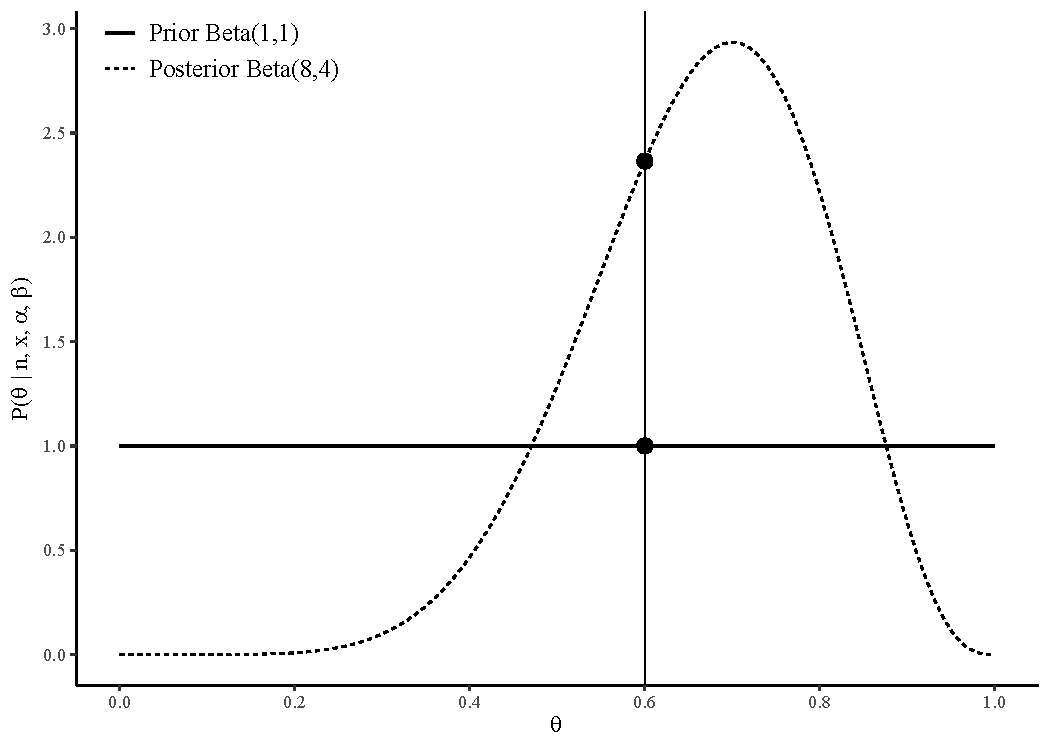
\includegraphics[width=12cm]{r-files-bes-klugkist-volker-2022/Figures/betaplot}}
 \caption{Prior $Beta(1,1)$ and the Posterior $Beta(8,4)$ after observing 7 successes in a sample of size 10.}
 \label{betaplot}
\end{figure}

To illustrate inequality constrained testing, we consider the hypothesis stating that the success probability is larger than 0.6.
This hypothesis is evaluated against the unconstrained, the complement, and the null hypothesis. In this relatively simple model, the Bayes factors can be computed analytically. Using Figure \ref{betaplot}, the calculation of each Bayes factor is explained. The plot shows the prior distribution, $Beta(1,1)$, as well as a posterior assuming that we observed a sample of size $n=10$ with number of successes $x=7$, providing $Beta(8,4)$.

\begin{table}[!h]
\caption{Posterior fit $f_j$ (for $H_i$ and $H_c$) or density at $\theta=0.6$ (for $H_0$), prior fit $c_j$ (for $H_i$ and $H_c$) or density at $\theta=0.6$ (for $H_0$) and Bayes factor for each hypothesis against $H_u$ (based on $Beta(1,1)$ prior for $\theta$ and $x=7$ successes in $n=10$ observations)}
\label{calcBF}
  \centering
     \begin{tabular}{lrrr}\hline
$H_j$                 & posterior   & prior  & $BF_{j,u}$   \\ \hline
$H_u: \theta$        & 1     & 1     & 1       \\
$H_i: \theta>0.6$    & .704  & .400  & 1.76    \\
$H_c: \theta<0.6$    & .296  & .600  & 0.49    \\
$H_0: \theta=0.6$    & 2.365 & 1.00  & 2.36    \\ \hline
\end{tabular}
\end{table}


For $BF_{i,u}$ and $BF_{c,u}$ we need to evaluate the parts of both the prior and the posterior distributions in agreement with the constraints of $H_i$ and $H_c$, respectively.
For $H_i$ this is the area to the right of the vertical line at $\theta=0.6$ in the prior and posterior distributions. For $H_c$ we need the two areas to the left of this vertical line.
The volume of the beta distribution that is in line with the constraints can, for instance, be calculated using the \verb"pbeta" function in \verb"R".
For $BF_{0,u}$ we use the Savage-Dickey density ratio method. In Figure \ref{betaplot}, the two large dots show the two densities that are required for this ratio: the prior and posterior density at $\theta=0.6$. These densities can, for instance, be obtained by the \verb"R" function \verb"dbeta". The resulting values for fit, complexity and the Bayes factor against the unconstrained model are provided in Table \ref{calcBF}.

From these results, the Bayes factors of interest (for $H_i$ against each of the alternatives) can easily be computed, as was explained before.
In Table \ref{Neffect}, the first column provides the results for the current scenario ($n=10$, $x=7$). The other columns demonstrate the behaviour of the different Bayes factors for increasing sample size (with the success rate fixed at 0.7 and thus in agreement with the hypothesis of interest $H_i$).


\begin{table}[!h]
\caption{Testing $H_i: \theta>0.6$ against $H_u$, $H_c$, and $H_0$ for increasing sample sizes $n$ and fixed observed success probability ($x/n=0.7$); all with prior $p(\theta)\sim Beta(1,1)$}
\label{Neffect}
  \centering
     \begin{tabular}{crrrrrrr}\hline
$n \rightarrow$  & 10    & 20    & 40   & 80   & 100  & 500  & 1000  \\ \hline
 $BF_{i,u}$  & 1.76  & 2.00  & 2.24 & 2.41 & 2.45 & 2.50 & 2.50  \\
 $BF_{i,c}$  & 3.56  & 5.99  & 12.72& 41.53& 70.69& 8.2E5  & 5.6E10   \\
 $BF_{i,0}$  & 0.74  & 0.77  & 0.95 & 1.73 & 2.42 & 6.3E3  & 2.2E8   \\ \hline
\end{tabular}
\end{table}

The results show that all three Bayes factors generally behave well with increasing support for $H_i$ when the sample size increases. However, we also see that $BF_{i,u}$ is bounded at a maximum of 2.50. The explanation is straightforward when considering the formula $BF_{i,u}=f_i/c_i$. With a result in agreement with $H_i$ and increasing sample size, at some point the entire posterior is in agreement with $H_i$, providing $f_i=1$, i.e., the maximum value for perfect fit. The Bayes factor is then determined by the complexity measure $c_i$ that does not depend on sample size and is equal to 0.4 in our example. The maximum $BF_{i,u}$ value is then 1/0.4 = 2.50. On the other hand, testing against the complement implies the comparison of hypotheses that describe two mutually exclusive parts of the parameter space. Thus, if the fit of $H_i$ approaches one, then the fit of $H_c$ approaches zero, and vice versa. Therefore, the evidence for the correct hypothesis renders infinite support with increasing sample size.

Another observation is that testing against the null hypothesis suffers from `power' problems when samples are small. In this example, for samples of 10, 20, or 40 observations, $BF_{i,0} < 1$, showing more support for $H_0$ than for $H_i$. The explanation is simple and very similar to what happens with NHST in the frequentist framework: the parsimoniousness of the null hypothesis (it has less parameters than any of the other models) benefits this model when deviations from the null are small compared to the amount of evidence (i.e., the sample size of the study).

These observations lead us to two general recommendations for two different situations. First, if the main goal is to evaluate one informative hypothesis and to what extent it is supported by the data, then it is recommended to use $BF_{i,c}$. It is the most powerful test and it does not have a maximum value, so, the more data in agreement with the hypothesis are observed, the more support the Bayes factor will show. Second, if multiple informative hypotheses are of interest, and specifically their mutual comparison, it is recommended to evaluate them against one another. One of these informative hypotheses could also be the null hypothesis but, when including the null, one needs to take into account that larger samples are required to have reasonable power to detect the true hypothesis if this is not the null. Whether a sample is sufficiently large depends on the number of parameters and the number and type of constraints and is, to the best of our knowledge, hardly studied in the context of informative hypothesis testing \citep[for an exception in the context of comparing two means, see][]{fu_sample_2021}.





\section{Aggregating evidence from multiple studies}\label{Multiple}

Replication is important and increasingly performed but it raises the question of how to aggregate results from multiple studies. As mentioned in the introduction, for \textit{close} replications there are several options due to high similarity between the resulting datasets in this context. However, when \textit{conceptual} replications are performed this may lead to datasets that vary in format and require different statistical models. For the latter, BES is proposed as an alternative tool for aggregating evidence.
We start this section with an introduction of BSU and BES and a comparison of methods for studies with data in the same format. This comparison is supported by illustrations using the binomial example of the previous section.
The final subsection provides an illustration of the synthesis of evidence from a set of \textit{conceptual} replications leading to data that cannot be aggregated using BSU. The studies to be synthesized come from the same underlying population (with known effect size) but consist of different data formats, that are therefore analyzed by different statistical models. Using an example with different types of regression models as the statistical analysis tools, we demonstrate that the BES approach does provide a measure for the combined amount of evidence. A few simulation studies are presented to get a first impression of what BES entails, how it works, and what potential limitations are.



\subsection{Bayesian sequential updating (BSU)}
BSU has been well described in the literature \citep[e.g.,][]{schonbrodt_sequential_2017, verhagen_bayesian_2014} and is a procedure that pools data either case by case or study by study. The key idea is that the current state of knowledge about a parameter or hypothesis can be computed at any moment in the data collection period. In the context of replication, data from a first study provides (after specifying an initial prior distribution) the posterior distribution, which is subsequently used as the prior distribution for a second study. After each study, the posterior distribution reflects the current state of knowledge about the model parameters. The method is coherent, meaning that, with the same initial prior distribution, the posterior after adding one set of 100 observations is exactly the same as the posterior after sequential updating, for instance, after every tenth observation. Also the order in which (subsets) of data come in does not affect the final resulting posterior.

Also, after each study, sequential Bayes factors (SBF) can be computed and reflect the current level of relative evidence for the hypotheses of interest. When used for null hypothesis testing (i.e., $BF_{1,0}$), with large enough sample sizes the SBF always converges to zero (if $H_0$ is true) or infinity (when $H_1$ is true), that is, it is \emph{consistent}. This does not automatically generalize to comparing other types of hypotheses with Bayes factors. For instance, when used for testing an order constrained hypothesis against the unconstrained hypothesis (i.e., $BF_{i,u}$), the SBF will converge to zero when $H_i$ is not true, but to a maximum value, determined by the complexity of the informative hypothesis, when $H_i$ is true (see also the previous section). However, it generally holds that by pooling the data from multiple studies, as is done with BSU, the overall power to detect true effects increases. As such, aggregating evidence with BSU can be a solution for power problems when the individual studies are small. In our context of comparing an informative hypothesis against the unconstrained, complement, or null alternative, the results when testing against the null hypothesis indeed showed that small, underpowered studies failed to find evidence for the true effect. Using a data pooling approach to basically increase the overall sample size increases the overall power to detect effects, which is clearly a major strength of the approach.

Another strength of BSU (compared to the NHST approach) is that a priori power analyses are not needed. Instead, one can specify a stopping rule, e.g., \textit{the resulting Bayes factor should be larger than 10 for one of the two compared hypotheses}. Data collection and evaluation of the hypotheses then continues until this threshold is reached (or resources are exhausted). This implies multiple or interim testing, that is, at several points in the data collection the SBF is calculated and based on the resulting value one either stops, or adds more data. Under the NHST framework such interim analyses require a correction for multiple testing. It is generally accepted that no penalty for multiple testing is required when computing the Bayes factor after each updating step. However, potential bias of Bayes factors in sequential designs is a topic of debate and long-term error rates can be affected by the SBF approach. Further elaboration is beyond the scope of this paper; interested readers are referred to \citet{schonbrodt_sequential_2017} and references cited herein.

Finally, there is a limitation of sequential updating and that is the high level of similarity that the studies to be aggregated must have. To use data pooling techniques (sequential updating is one example, meta-analysis another), the data must have a similar format, because the synthesis takes place at the level of the model parameters or functions of parameters, like effect sizes. For highly diverse studies like those that could result from conceptual replications, we need a more flexible approach.





\subsection{Bayesian evidence synthesis (BES)}

In the context of conceptual replications, a theory of interest is investigated with studies that are substantially different. These differences can lead to data sets of different formats and a subsequent need for different statistical models with different parameters. This diversity between studies makes data pooling or aggregation on the level of parameters complex and often impossible. In those cases BES can serve as an alternative.

The BES approach assumes that multiple studies exist that investigate a common general theory but may be so diverse in design and measurements, that also the study-specific informative hypotheses reflecting this common theory can differ. To give just one example, consider three studies that all involve the same concept of interest (e.g., as predictor in a regression context) but in one study this concept was measured with a continuous variable, in a second study with a categorical variable with three levels, and in a third study with a categorical variable with five levels. This would lead to different statistical models and also to different constraints on the corresponding model parameters. However, in each study, Bayes factors can be computed to measure the support for the study-specific informative hypothesis. Given that, in each study, the informative hypothesis does reflect the common theory of interest, BES can be used to meaningfully combine the Bayes factors.

The idea is to first quantify the evidence for or against the hypothesis of interest in each individual study and then pool the evidence over studies, providing a joint level of support for the general theory.
The aggregation is based on updating model probabilities using Eq.\ref{odds}, that is, the posterior odds after observing a first data set are used as the prior odds for the second study; and the posterior odds after inclusion of the second study are used as the prior odds for the third study. This process can be repeated for each new data set, or each additional replication study as presented in:
\begin{equation}\label{aggrodds}
  \Bigg(\frac{P(H_1|D)}{P(H_2|D)}\Bigg)^T = \frac{P(H_1)}{P(H_2)} \prod_{t=1}^{T}{(BF_{1,2})^t},
\end{equation}
where $t=1, \ldots, T$ indicates the number of studies. Note that the prior odds before the first study $P(H_1)/P(H_2)$ in Eq.\ref{aggrodds} is often set to one, reflecting no preference for either hypothesis before any data was observed. But, if desired, any other prior odds can be included. Also note the simplicity of the computation of aggregated evidence from $T$ studies; it is simply the product of the Bayes factors from the individual studies, weighted with the initial prior odds.

There is related prior work where aggregation at the level of Bayes factors is proposed and investigated. In the context of neuroimaging, \citet{stephan_gbf_2007} and \citet{stephan_gbf_2009} describe what they call pooled Bayes factors (comparable to BSU) and group Bayes factors (comparable to BES) to combine evidence for a set of models of interest from multiple subjects in a within-subjects design \citep[see also][who discuss these methods]{regenwetter_heterogeneity_2018}. The group Bayes factor (GBF) assumes independence of the subjects and are computed as the product of individual evidence levels (Bayes factors) to obtain the aggregated support for a model. Also, \citet[][]{klaassen_all_2018} investigated the use of Bayes factors to aggregate evidence over multiple $N=1$ studies.

Also in BES, the underlying assumption is that all studies provide independent information about the general theory of interest. It is important to note that it is, therefore, \emph{not} a data pooling approach and thus essentially different from Bayesian updating. It is an alternative way of combining evidence levels from a set of studies, necessarily also leading to different interpretations of results. Whereas BSU investigates to what extent \emph{all data together} provide evidence for a hypothesis of interest, BES provides the level of evidence for the extent to which a hypothesis is supported in \emph{each of the studies}.

Linking the two approaches would require simultaneously updating the parameter distributions and the model odds in the BES approach. 
So, after one study the posterior odds are used as prior odds for the next study, but also the posterior parameter distribution is used as the prior parameter distribution for the next study.
If this is done, Eq.\ref{aggrodds} provides the same results as obtained when calculting the Bayes factor after sequential updating. 
A small numerical illustration is given in the next section.
However, when studies apply different statistical models with different model parameters this cannot be done. In those cases, that is where BSU is not feasible, BES offers an alternative, albeit with a different synthesis question (and thus different results).

In conclusion, BES can aggregate evidence from studies that cannot easily be aggregated with other methods like BSU or meta-analysis. In the context of conceptual replications the BES approach fits very well and provides answers to a useful question, that is, what is the overall, combined level of support for a hypothesis when investigated with studies that are related but not similar. If the hypothesized effect finds support when combining the support levels in all these studies, then it can be concluded that the results are robust with respect to (perhaps arbitrary) study design choices. So, BES provides a flexible tool that can synthesize evidence from studies even when they are highly diverse and answers a research question that is relevant for conceptual replications.

However, it is also important to mention limitations of BES, especially when compared to BSU or meta-analysis. Because BES is not a data-pooling method, aggregation over multiple studies does not increase the power to find support for a hypothesized effect. One of the goals of combining studies is to overcome a lack of power of individual studies, especially when the individual studies, or effect sizes of interest, are relatively small. This is not accomplished with BES, as we also demonstrate in the next section. Another goal of combining studies may be to inspect the effect of moderators, that is, study characteristics that may affect the effect size of interest. This is a strength of meta-analysis, where in mixed effects models (or meta regression) study-level variables can be included as predictors for effect sizes \citep[e.g.][]{Borenstein2009}. It would be interesting to explore methods to study heterogeneity in study results under the BES framework presented here but, to the best of our knowledge, this has not been done yet.




\subsection{Aggregation in the binomial example}\label{Binmultiple}

To assess how BES performs and to show the differences with BSU, we compare results from aggregation using BSU and BES in the same binomial example as used before.
We evaluate the informative hypothesis $H_i: \theta>0.6$ by aggregating evidence from 1 to 5 studies, where each study has a sample size of 20 and an observed success probability of 0.7. As in the previous example, we use a $Beta(1,1)$ prior distribution. In Figure \ref{Aggregated}, the evaluation of $H_i$ against one of three alternative hypotheses is presented: the unconstrained model $H_u: \theta$ (left panel), the complementary model $H_c: \theta<0.6$ (centre panel), and the null model $H_0: \theta=0.6$ (right panel). Results are presented as posterior model probabilities (PMP) for $H_i$ after each additional study, using equal initial prior model probabilities.


\begin{figure}[ht]
   \centerline{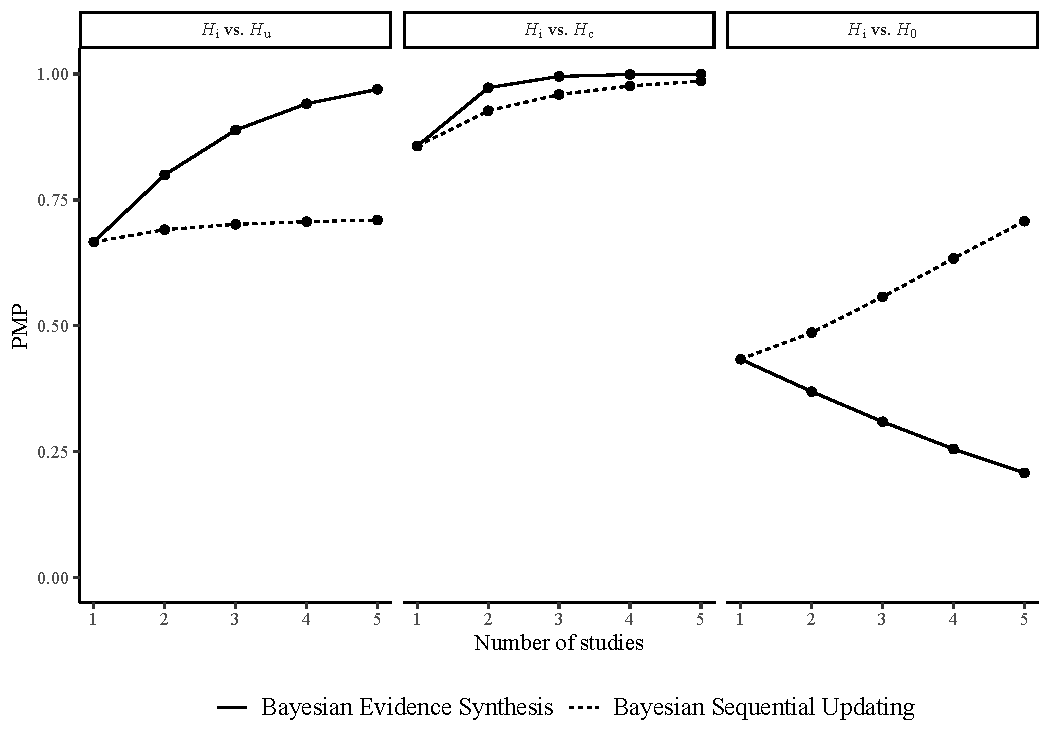
\includegraphics[width=14cm]{r-files-bes-klugkist-volker-2022/Figures/bes_bsu_7_pmp}}
 \caption{PMPs for BES (solid lines) and BSU (dashed lines) after combining 1-5 studies of $n=20$ and $x/n=0.7$ per study. All PMPs are the result of evaluating $H_i: \theta>0.6$ against one of the alternatives. Left panel: $H_u: \theta$. Centre panel: $H_c: \theta<0.6$. Right panel: $H_0: \theta=0.6$.}
 \label{Aggregated}
\end{figure}


It is clear that the two approaches indeed provide different results. When testing against the unconstrained model, BSU still has a maximum value determined by the complexity of the constrained hypothesis, irrespective of the number of studies. When there is enough evidence to reach a fit-value of one, the SBF for the pooled data can still not increase beyond 1/complexity; in our example 1/0.4=2.5 (PMP=0.71), which explains the almost horizontal dashed line in the panel on the left. BES, on the other hand, aggregates the amount of support for $H_i$ versus the alternatives in each study and then combines all pieces of evidence into one aggregate measure. Since every single study shows a preference for $H_i$ compared to $H_u$ ($BF_{i,u}=2$), the synthesized evidence for $H_i$ over multiple studies increases with each additional study, as can be seen by the steadily increasing solid line in this plot. In the centre panel, both synthesis methods show an increase in the aggregated PMP with an increasing number of studies that support $H_i$. Again the small differences in results between the approaches are caused by the fact that a different synthesis question is answered. This becomes even clearer in the right-hand panel, where $H_i$ is evaluated against $H_0$, while each individual study does not have enough power to show preference for $H_i$ over the more parsimonious model $H_0$. In this scenario, BSU shows an increasing amount of evidence for $H_i$ when adding additional studies. The data pooling approach achieves that at some point there is enough power to find more support for the informative hypothesis than for the null hypothesis. This is not the case for BES, because the question answered by BES is about the support for $H_i$ in each individual study. Because each individual study prefers the simpler $H_0$, the aggregated evidence for $H_0$ becomes stronger with each additional study. This explains the decreasing solid line for the declining support for $H_i$.

To get further insight in the behaviour of aggregated evidence using BSU and BES, similar plots are constructed for data with different success probabilities. We start with a sample success rate of 0.8, again supporting the informative hypothesis of interest, but with more power due to a larger effect. Then we investigate results when the sample supports the null hypothesis, that is, a success rate of 0.6, and finally when the complement is supported with a success rate of 0.4. The same prior specifications are used, each study still has a sample size of $n=20$, and 5 identical studies are aggregated.


\begin{figure}[!ht]
   \centerline{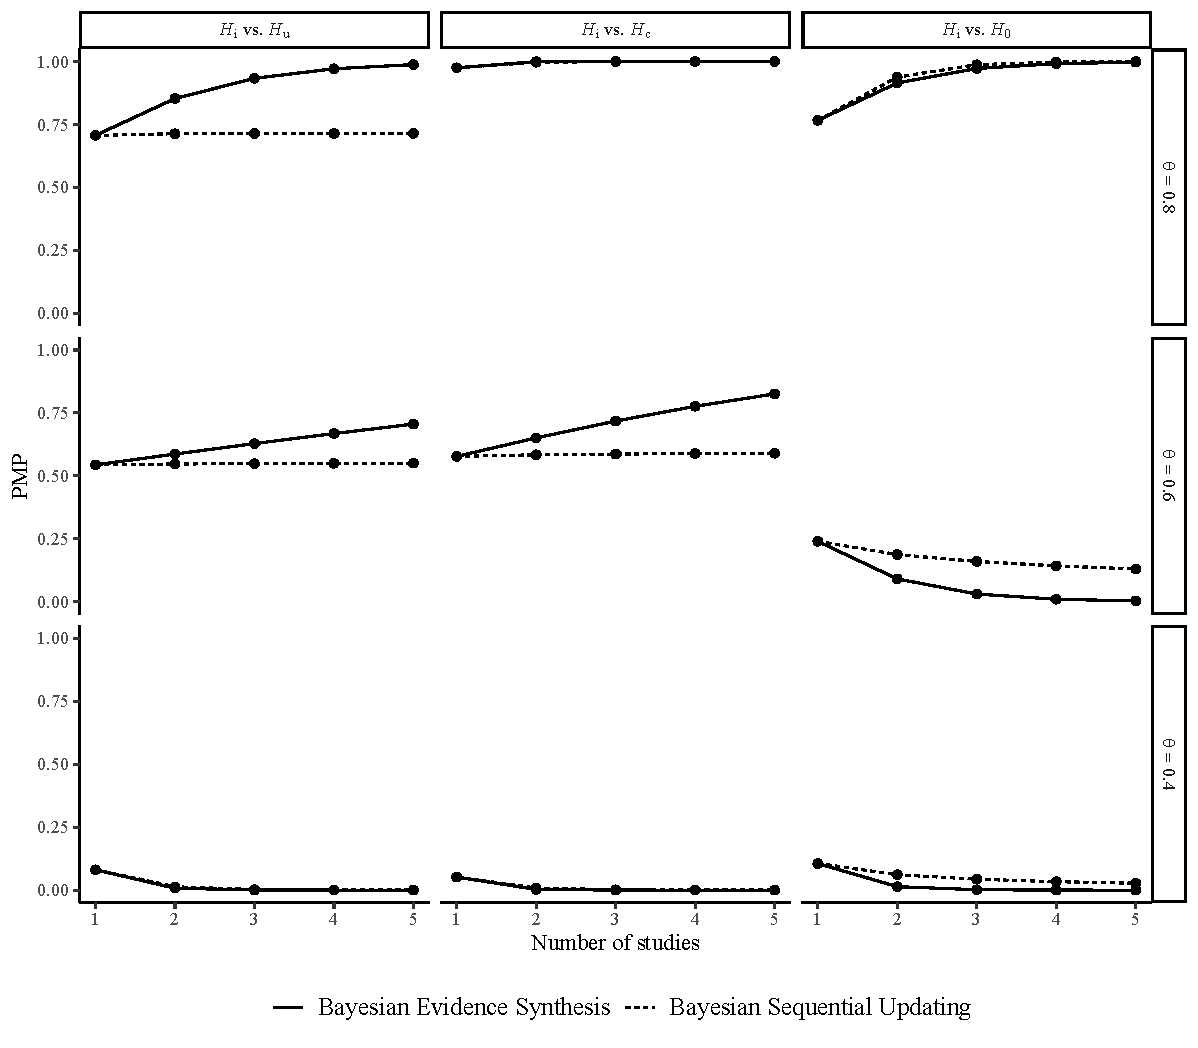
\includegraphics[width=14cm]{r-files-bes-klugkist-volker-2022/Figures/bes_bsu_pmp}}
 \caption{PMPs for BES (solid lines) and BSU (dashed lines) after combining 1-5 studies of $n=20$ with different effect sizes per row and testing $H_i: \theta>0.6$ against one of the alternatives $H_u: \theta$ (left), $H_c: \theta \leq 0.6$ (centre), $H_0: \theta=0.6$ (right). In the top row: $x/n=0.8$ and thus in agreement with $H_i$. In the middle row: $x/n=0.6$ and thus in agreement with $H_0$. In the bottom row: $x/n=0.4$ and thus in agreement with $H_c$.}
 \label{aggre2}
\end{figure}

In Figure \ref{aggre2}, in the top row, results are plotted for the aggregation of evidence from 1 to 5 studies with success probability 0.8, that is, the data per study are in agreement with $H_i: \theta>0.6$. The increasing solid lines in the left, centre and right plot show the increasing amount of aggregated support when using BES with each of the three alternative hypotheses ($H_u$, $H_c$, $H_0$). We see that the current combination of effect size and sample size provides enough power for testing against $H_0$ in each study, and therefore also the aggregated support for $H_i$ increases with each new study. In the central plot on the first row, the almost horizontal line for testing against $H_c$ demonstrates that the support for $H_i$ against $H_c$ in this scenario approaches maximal support already with less than 5 studies.
Comparing the results with BSU, the dashed lines in the same plots, we see only a difference when evaluating against $H_u$. This is, again, explained by having a maximum value for the Bayes factor (and PMP) when testing against an unconstrained model.

In the middle row, the observed effect in each sample is 0.6, which conforms exactly to the null hypothesis $H_0: \theta=0.6$. BSU results when testing against $H_u$ (left) or against $H_c$ (centre) show a stable indecisive result irrespective of adding more studies (horizontal dashed lines at PMP $\approx .5$). In contrast, BES shows a small increase in aggregated support for $H_i$ when adding more studies. Since $H_i$ is not 'the correct' hypothesis one could consider this an undesired result. The explanation is found in the fact that a Bayes factor balances fit and complexity and the two hypotheses compared (for both alternatives) differ in specificity. This is easiest explained by looking at testing $H_i$ against $H_c$ (centre plot). The sample results with observed success rate of 0.6 provide approximately equal support, in terms of fit of data to the hypothesis, for $\theta>.6$ and $\theta<.6$. But $H_i: \theta>.6$ is more specific (containing 40$\%$ of the prior space) than $H_c$ (containing 60$\%$). This specificity effect accumulates over studies using BES, but not using BSU. In the plot on the right, both BSU and BES show declining support for $H_i$ when tested against the in the data supported $H_0$. The gain in support in favor of the null hypothesis after synthesizing up to 5 studies is larger for BES than for BSU.

The bottom row presents the synthesized results when each study has success probability 0.4, that is, a result not in agreement with $H_i$, but instead in agreement with $H_c$. Irrespective of the alternative hypothesis, there is little support for $H_i$, as one would expect since each of the alternatives is more in line with the data than $H_i$ is. Both BSU and BES also show a further decrease in PMP values when adding more studies.

As a last comparison between results from BSU and BES in a context where both could be applied (i.e., each study has the exact same model, parameter and hypothesis of interest), we show how the product of Bayes factors as used in BES yields the same results as BSU when the (unconstrained) parameter distributions are also updated after each new study.
Let us consider combining two studies of size $n=10$ with 7 successes in each study and testing $H_i: \theta>0.6$ against the unconstrained alternative. The initial prior used is again the $Beta(1,1)$. BSU pools all available data and thus results in a Bayes factor corresponding to 14 successes in a sample of 20, providing $BF_{i,u}=2.00$ (a result that can be found in Table \ref{Neffect}; first row, second column).
With BES, the first study provides the posterior $Beta(8,4)$ and $BF_{i,u}=1.76$ (see also Figure \ref{betaplot} and Tables \ref{calcBF} and \ref{Neffect}). Using $Beta(8,4)$ as the prior distribution for the second study provides a posterior distribution equal to a $Beta(15,7)$ (that is, the new study adds 7 successes and 3 failures). Evaluating the prior and posterior in the second study results in $c_i=0.70$ and $f_i=0.80$ and subsequent $BF_{i,u} = 1.14$. Now, the product of Bayes factors (1.76*1.14) indeed obtains the value 2.00, that is, the same result as with BSU.




\subsection{An example of conceptual replications}\label{GLMexample}

In the previous section, we gave examples in which both BSU and BES could be applied.
However, as previously discussed, when studies are methodologically diverse, using, for example, different operationalizations of key variables or different statistical models, BSU becomes inapplicable due to the fact that the estimated parameters are incomparable.
Meta-analysis allows for some heterogeneity between studies, but also becomes infeasible when the estimated parameters cannot be converted into a common effect size. 
For example, it might be the case that both the measurement levels of predictor (e.g., continuous versus ordinal with three levels) and outcome variables (e.g., continuous versus dichotomous) are different between studies, rendering BSU and meta-analysis infeasible.
However, if the underlying theory is the same in all studies, it is straightforward to quantify the support for the corresponding hypotheses in all studies, and aggregate the overall amount of evidence with BES. In the upcoming section, we present two simulation examples with such different operationalizations, both conducted in \texttt{R} \citep[][Version 4.2.1]{R}.

\subsubsection{Simulation 1: Using BES when studies have different outcome variables}


In the first simulation, data is generated to represent three different studies using three different statistical models: ordinary least squares (OLS), logistic and probit regression.
In each study, a continuous or binary outcome $Y$ is regressed on five predictor variables $X_k$ ($k = 1,2,3,4,5$), that are normally distributed with mean $\mu_k = 0$, variance $\sigma^2_{k} = 1$ and common covariance $\rho_{k,k'} = 0.3$.
We consider the sample sizes $n = (50, 100, 200, 400, 800)$, and effect sizes $R^2 = (0.02, 0.09, 0.25)$, in accordance with small, medium and large effects, respectively, as defined by \citet{cohen_1988}.
When the outcome of the study is continuous, the conventional $R^2$ is used, while for binary outcomes, McKelvey and Zavoina's $R^2_{M\&K}$ \citep*{mckelvey_zavoina_1975} is used.
In each study, the relation between the predictors and the outcome variable is defined such that $\beta_1 = \beta_2 = \beta_3$, $\beta_4 = 2 \beta_1$ and $\beta_5 = 3\beta_1$.
The exact sizes of the coefficients depend on the effect size and the regression model used to generate the data (Appendix \ref{appendix:gendat} details how to calculate the coefficients for each model and effect size).
Based on the predictor variables and regression coefficients, the continuous outcomes are drawn from a normal distribution.
For dichotomous outcomes, the predictor variables and regression coefficients are first used to obtain success probabilities for each individual, after which the outcomes are drawn from a Bernoulli distribution (the exact procedure is described in Appendix \ref{appendix:gendat}).

For all combinations of effect and sample size, data is generated using OLS, logistic and probit regression models, to reflect three different studies.
In each of these studies, the focus is on the last three predictors, and the hypothesis $H_1: \beta_3 < \beta_4 < \beta_5$ is evaluated against its complement \citep[using the \texttt{BF()} function from the \texttt{R}-package \texttt{BFpack}, with default (prior) settings;][Version 1.0.0]{BFpack}.
Subsequently, BES is used to aggregate the evidence for $H_1$ over these three studies.
The initial prior model probabilities are specified equally (i.e., $P(H_1) = P(H_{c}) = 0.5$).
This procedure is repeated over 1000 iterations for each combination of effect and sample size, to prevent that random fluctuations in data generation affect the conclusions.
The results are reported visually, in terms of the aggregated posterior model probabilities after incorporating the evidence from each of the three studies.
In these simulations, a combined PMP that is greater than $0.5$ reflects more support for the true hypothesis $H_1$ than for its complement $H_c$.

\begin{figure}[ht]
   \centerline{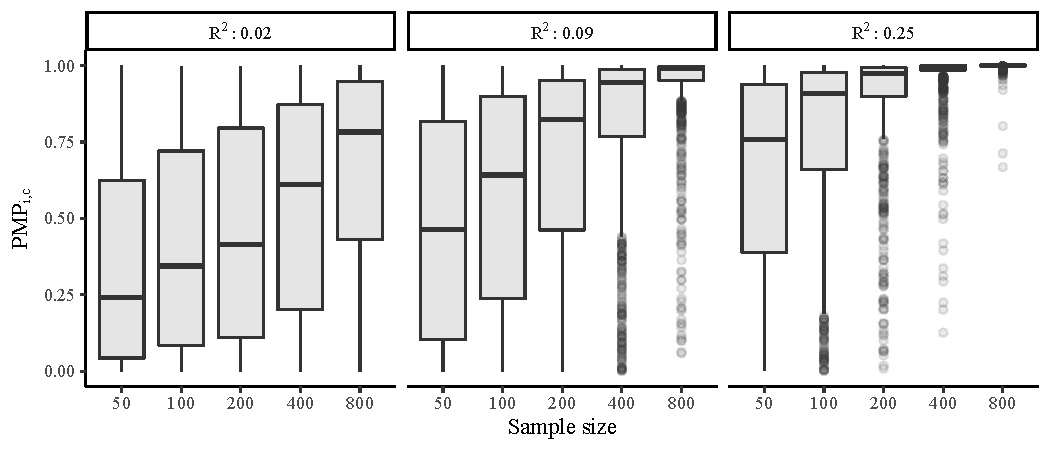
\includegraphics[width=15cm]{r-files-bes-klugkist-volker-2022/Figures/sim1_box}}
 \caption{Aggregated PMPs for the evidence for hypothesis $H_1: \beta_3 < \beta_4 < \beta_5$ against $H_c$ over three studies (based on OLS, logistic and probit regression models) for different combinations of effect and sample size.}
 \label{sim1_box}
\end{figure}

Figure \ref{sim1_box} shows that the support for the true hypothesis $H_1$ provided by BES increases with effect and sample size.
When the effect size is small, the support for $H_1$ varies considerably over the iterations, but hardly ever reaches convincing levels.
The same is true for the smallest sample size and a medium effect.
In these scenarios, each of the individual studies lack statistical power, regardless of the model used to generate the data.
For example, in Table \ref{pmp-studies} it is shown that the combination of the smallest effect size and smallest sample size yields a median PMP of about $.43$ in the individual studies (over 1000 iterations), with equivalent results for all three regression models.
Consequently, each of the studies contributes some support \textit{against} the hypothesis of interest, which accumulates when aggregating over studies.
Hence, when evaluating hypotheses on multiple parameters, BES requires sufficient statistical power, also when the alternative hypothesis of interest is not a classical null hypothesis (as presented in Section \ref{Binmultiple}) but a more general alternative hypothesis.
When the effect and sample sizes of the individual studies are sufficiently large, the aggregated support for $H_1$ is concentrated close to $1$, while there are less and less iterations that find little to no support.
Overall, these results again highlight that a lack of power in the individual studies accumulates when using BES.
When studies have sufficient power, BES can be applied to aggregate the evidence for theoretically equivalent hypotheses over heterogeneous studies.


\subsubsection{Simulation 2: Using BES when the studies have different predictors and outcome variables}

Simulation 2 builds on simulation 1, using the same sample sizes and effect sizes.
The outcome $Y$ is again continuous or binary, and is generated on the basis of the five predictor variables $X_1$ to $X_5$ using OLS, logistic and probit regression models.
The predictors of interest differ from simulation 1, as the focus is now on $X_1$, $X_2$ and $X_3$.
Moreover, simulation 2 exemplifies how BES can be used when not only the measurement level of the outcome variables, but also the operationalizations of the predictor variables differ.
Regardless of the operationalizations, which are manipulated after generating the data, it is assumed that $X_1$, $X_2$ and $X_3$ are different indicators of the same construct that is positively related to the outcome $Y$ ($H_2$).

In study $a$ the OLS model is used. Here, we consider the three distinct predictors separately, and thus hypothesize that $H_{2a}: \{\beta_1, \beta_2, \beta_3\} > 0$.
Study $b$ applies the logistic regression model. The three indicators are transformed into a scale score, by taking the mean of the three indicators for each observation, which is a common approach in the social sciences \citep[e.g.,][]{bauer_discrepancy_2016}.
The corresponding hypothesis is that this scale score is positively related to the outcome $Y$, which yields $H_{2b}: \beta_{\text{scale}} > 0$.
In study $c$, generated and analyzed with probit regression, this operationalization is further adjusted.
The scale score that is used in study $b$ is categorized into three equally sized groups in each sample, corresponding to a \textit{low}, \textit{medium} and \textit{high} scoring group.
This is, despite advice against it, common practice in many areas of research \citep[e.g.,][]{bennette_against_2012, decoster_best_2011}, or it may simply be a consequence of how the data is collected.
The same expected positive relation between predictor and outcome now yields a specific ordering in the group means, resulting in hypothesis $H_{2c}: \beta_{\text{low}} < \beta_{\text{medium}} < \beta_{\text{high}}$.


\begin{figure}[ht]
   \centerline{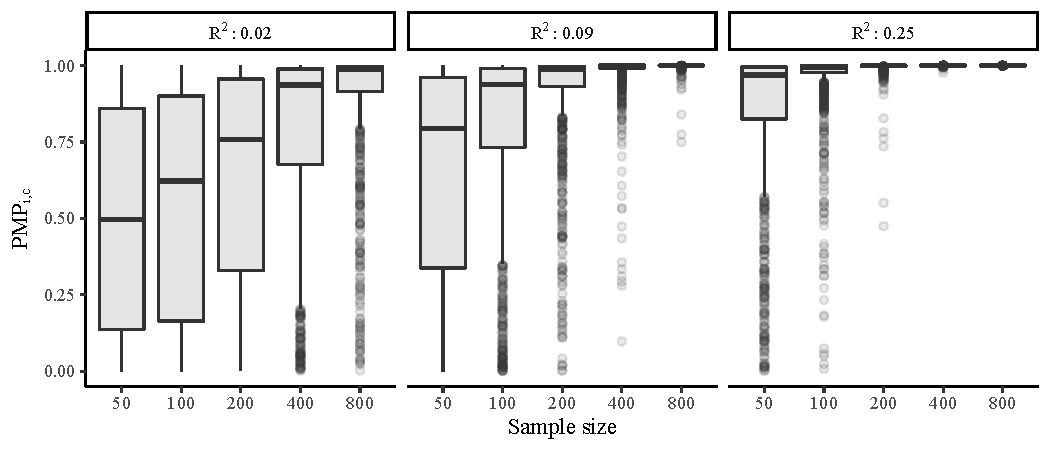
\includegraphics[width=14cm]{r-files-bes-klugkist-volker-2022/Figures/sim2_box}}
 \caption{Aggregated PMPs for the evidence for hypotheses $H_{2a}: \{\beta_1, \beta_2, \beta_3\} > 0$, $H_{2b}: \beta_{\text{scale}} > 0$ and $H_{2c}: \beta_{\text{low}} < \beta_{\text{medium}} < \beta_{\text{high}}$ against their respective complements over three studies (based on OLS, logistic and probit regression models) for different combinations of effect and sample size.}
\label{sim2_box}
\end{figure}


In simulation 2, the aggregated support for $H_2$ exceeds the support for its complement in the majority of the simulations for all effect and sample sizes, except for the combination of the smallest effect size with the smallest sample size.
In the latter case, the evidence is indecisive, with about equal support for both the hypothesis of interest and its complement.
The aggregated evidence for $H_2$ increases with effect size and sample size, and reaches substantial levels from relatively small sample and effect sizes onward.
For the largest effect size, the vast majority of the simulations results in relatively strong evidence for the overall hypothesis for all sample sizes.
Hence, although the study-specific hypotheses differ from study to study, the aggregated evidence supports the overall theory.


However, the aggregated results do not reveal how the individual studies contribute to this aggregate.
Whereas in the previous simulations, the considered hypothesis was identical over the different studies, the operationalization of the construct of interest, and thus the hypothesis under evaluation now varies over the three studies.
The hypotheses differ in the type and number of constraints, and therefore have different complexities.
At the same time, the different operationalizations affect the power of the performed analyses within each study.
Comparing the contributions of the individual studies indeed reveals that some operationalizations provide higher levels of support for the overall hypothesis than others (Table \ref{pmp-studies}).
Consistently over all combinations of effect and sample size, the data generated and analyzed with the logistic model, in which the separate indicators were averaged as a scale score, yielded the highest posterior model probabilities, and therefore contributed more to the aggregated evidence than the studies with OLS and probit data.
For example, for the smallest effect size and the smallest sample size in simulation 2, both the OLS and the probit study provide more support for the respective complement hypotheses, whereas only the logistic study provides evidence for the hypothesis of interest.
These results show that different ways of operationalizing the same theoretical construct affect the outcomes, but the final measure of BES does not reflect this variability. Hence, the individual studies provide valuable additional information.


\begin{table}[t]
\caption{Median posterior model probabilities for the individual studies and aggregated over studies in simulation 1 and 2, for a selection of effect sizes and sample sizes.}
\label{pmp-studies}
\centering
\begin{tabular}{lrrrrrrr}
\hline
Simulation & $R^2$ & Sample size & OLS & Logistic & Probit & & Aggregated \\
\hline
1 & $0.02$ & 50 & 0.44 & 0.43 & 0.42 & & 0.24 \\
  & $0.02$ & 200 & 0.52 & 0.50 & 0.50 & & 0.42 \\
  & $0.02$ & 800 & 0.65 & 0.61 & 0.62 & & 0.78 \\
\hline
1 & $0.25$ & 50 & 0.66 & 0.61 & 0.59 & & 0.76 \\
  & $0.25$ & 200 & 0.81 & 0.79 & 0.76 & & 0.97 \\
  & $0.25$ & 800 & 0.96 & 0.93 & 0.91 & & 1.00 \\
\hline
2 & $0.02$ & 50 & 0.45 & 0.62 & 0.49 & & 0.50 \\
  & $0.02$ & 200 & 0.58 & 0.69 & 0.54 & & 0.76 \\
  & $0.02$ & 800 & 0.75 & 0.90 & 0.71 & & 0.99 \\
\hline
2 & $0.25$ & 50 & 0.75 & 0.87 & 0.65 & & 0.97 \\
  & $0.25$ & 200 & 0.93 & 0.98 & 0.86 & & 1.00 \\
  & $0.25$ & 800 & 1.00 & 1.00 & 0.98 & & 1.00 \\
\hline
\end{tabular}
\end{table}


\section{Conclusion and discussion}
\label{Concl}

In this paper we introduced BES as an alternative method for combining results from multiple studies. 
Before discussing opportunities and limitations of BES, it is important to describe how it is essentially different from BSU and meta-analysis.
The latter methods pool the data (or summaries of the data) in order to obtain a level of evidence when taking data from all studies together. In our context of using Bayes factors to evaluate an informative hypothesis, BSU assumes that the hypothesis and relevant model parameters are identical in all studies. The resulting Bayes factor provides the information how much more likely it is that the informative hypothesis is true compared to the alternative, taking all data together. As such, BSU gains power by combining observations from multiple studies. When the assumption of equal models and hypotheses between studies hold, as for instance in the context of exact replication studies, we recommend using BSU and the SBF; it is consistent, coherent, and may overcome power issues in individual studies.

Meta-analysis is another data pooling approach and thus also has the potential to solve power issues.
Compared to BSU, it is more flexible with respect to differences between studies. 
As long as the effect sizes obtained in the individual studies are comparable, or can be converted into a comparable measure, meta-analysis can be used to pool the results.
In addition, meta-analysis provides the option to study heterogeneity in results by including study level predictors and investigate how variation between study effect sizes can be understood. Finally, within the meta-analysis literature there is ample attention to the problem of publication bias and how the distribution of effect sizes in a meta-analysis can indicate whether such problems are likely. When feasible to apply, meta-analysis therefore also has several benefits. 

In contrast with BSU and meta-analysis, BES is \emph{not} a data pooling approach and therefore lacks some of the advantages of the other approaches. However, it provides a tool that can synthesize evidence from studies that cannot be synthesized with BSU or meta-analysis because they do not share the same model parameters, or model parameters that can be made comparable. Such studies could typically result from conceptual replications, where variability in research designs, for instance in terms of operationalizations of key constructs and analysis models, is encouraged to enhance the validity of the drawn conclusions. In such a context, BES provides a flexible alternative to conventional approaches for a quantitative synthesis of the evidence for the overall theory.

There are two assumptions underlying the BES approach. First, all target studies must investigate the same underlying common theory. Second, all these studies are considered to provide an independent piece of evidence for this underlying common theory.
As long as the common theory of interest can be formalized as an informative hypothesis, the support for the theory in each study can be expressed in terms of a Bayes factor comparing the support for the target hypothesis and the chosen competitor. Importantly, the informative hypotheses may differ from study to study as a consequence of using different study designs, or differently measured constructs. This may lead to different model parameters and thus to different constraints on parameters to reflect the underlying general theory. Assuming that each study individually contributes to the overall level of support for this general theory allows us to aggregate at the level of Bayes factors, which is what BES does.



To illustrate the behavior of BES we first demonstrated the aggregation of multiple studies with the same data format in each study. The presented scenario represents the situation of exact replications and therefore allowed for a comparison of results from BES with BSU. Using a simple binomial model that could be analyzed analytically, and multiple datasets with equal and known effects, we computed Bayes factors for an informative hypothesis against one of three typical alternatives: the unconstrained, the complement and the null hypothesis.

The results demonstrated that BES behaves well in the sense that larger sample sizes, larger effect sizes, and more aggregated studies generally increase the support for the best hypothesis. However, we also demonstrated that the two methods of aggregation, BES versus BSU, provide answers to different questions. As stated before, BSU pools all available data and thus provides the support for the hypothesis of interest in all studies when taken together. This increases the total sample size and thus statistical power to find support for the true hypothesis, and as such quantifies the available evidence in a coherent way. BES, on the other hand, measures the level of aggregated evidence differently, by first determining the evidence in each study and then combining the support levels over studies. This implies, for instance, that if two underpowered studies each provide most support for the null hypothesis, the aggregated evidence using BES results in even stronger support for the null, that is, BES is not a remedy against underpoweredness.

The strength of BES is its flexibility. Results of highly diverse studies can be aggregated in a simple straightforward way by updating posterior odds with each additional study. This was demonstrated in the two simulation studies in this paper. In the first simulation, the three studies that were aggregated differed in the outcome variable and corresponding statistical model, while the formulation of the informative hypothesis was equal for all studies. Repeated sampling of data representing these three studies and, in each repetition, aggregating evidence over the three studies demonstrated that BES can indeed aggregate evidence from diverse studies and showed, again, that the performance of BES is generally as one would expect. Larger samples and larger effect sizes lead to higher levels of support for the hypothesis that reflects the true population effect. It also showed that a lack of power in the individual studies accumulates when using BES. Where in the `one parameter with one constraint' binomial example, we only encountered power issues for testing against the null hypothesis, this simulation with a hypothesis with multiple constrained parameters showed similar issues when testing against a more general alternative hypothesis.

The second simulation used a similar set-up for sampling data for the different statistical models but now also changed the formulation of predictors, in such a way that different informative hypotheses represented the general hypothesis. The results showed that with these different operationalizations, some studies provided higher levels of support for the theory than others. For example, collapsing the three indicators into a single scale score increased the statistical power of the analysis, and thus contributed more strongly to the aggregated evidence than the study that included the separate indicators. Another difference between the hypotheses of the individual studies was the number of constraints imposed on the regression parameters, in order to represent the general theory of interest. Since the type and number of constraints determine the complexity of a hypothesis, and since the Bayes factor depends not only on the fit of the data to the hypothesis but also on this complexity, these differences have an impact on the level of support reached within a study. Table 3 in this paper gives a first impression of the impact of differences in informative hypotheses on resulting Bayes factors, but more research into this effect and to what extent this may be problematic for the aggregation is needed.

In conclusion, we believe that BES provides a valuable and unique tool for the aggregation of evidence from a heterogenous set of studies. It generally performs well, although certain issues require further attention.
The simulation studies in this paper were merely for illustrative purposes to get an impression on what BES has to offer, however, they also provided cues on what still needs to be investigated further in a more comprehensive evaluation of the performance of BES. For instance, users need to be aware that if one or more of the aggregated studies lack power, BES does not provide a solution for this underpoweredness because it is not a data-pooling approach. The Bayes factor in the underpowered study will provide most support for the most parsimonious hypothesis, and BES will take that support measure into account when aggregating evidence from multiple studies. A second issue that needs attention is that Bayes factors are not only affected by the fit of the data to the hypothesis (including the impact of effect sizes and sample sizes) but also by the complexity of the hypothesis. This principle of parsimony is generally known and understood when evaluating hypotheses with a single study. However, in the context of combining evidence levels from multiple studies, which do investigate the same underlying theory but may have different study specific hypotheses, the role of complexity is more complex. Study specific informative hypotheses that have a smaller complexity compared to other studies in the set will, with the same fit, provide larger Bayes factor values and thus have a stronger impact on the aggregated evidence. To what extent or under which circumstances this is desirable, or problematic requires more research into different scenarios. Also, the impact of aggregating studies with considerable differences in sample size is a relevant topic for future research. In the examples and simulations of this paper, we always aggregated evidence levels from studies of the same size. In practical applications, this is usually not the case and it is important to understand how this impacts the behavior of BES.

Our final remark is about the position of this paper in the existing literature. Although we consider this work to be an introduction of the BES approach and have written it for potential users who are new to the method, it is not the first paper about BES. It all started with the work by \citet{kuiper_combining_2013}. They introduced the method for the evaluation of a hypothesis constraining one regression parameter to be positive within different statistical models, applied in the context of sociological research. Since then, BES has been applied in a few psychological studies \citep{zondervan_parental_2019, zondervan_robust_2020, kevenaar_bes_2021} and a sociological study \citep{volker_cooperation_2022}, and is described in a paper providing an overview of different methods using Bayes factors \citep{heck_review_2022}. Only recently, we started studying BES under more varied circumstances to better understand its behavior. This led to two more papers written more or less in parallel with this introductory paper \citep[][both submitted for publication]{vanwonderen_bes_2022, volker_bes_2022}. We feel that to be able to properly evaluate and value BES, the current paper provides a good starting point.





\bibliography{bes.bib}
\bibliographystyle{apalike}


\begin{appendices}
\section{Data generation and analysis} \label{appendix:gendat}

In this appendix, the data-generating mechanisms of the two simulations are outlined in more (mathematical) detail.

\subsection{Simulation 1}

In simulation 1, data is generated to represent three different studies with different outcome variables, but with the same set of predictor variables.
For each of these three studies, a different statistical model is used to generate the data: ordinary least squares (OLS), logistic and probit regression.
Under OLS, the outcome variable $Y$ is continuous, whereas for logistic and probit regression, $Y$ is binary.
In each study, $Y$ is related to the $n \times 5$ predictor matrix $X$, where each predictor $X_k$
is normally distributed with mean $\mu_k = 0$, variance $\sigma_k^2 = 1$ and common covariance $\rho_{k, k'} = 0.3$.
Accordingly, the mean vector $\mu$ and covariance matrix $\Sigma$ are defined as
\begin{equation}
\mu = \begin{bmatrix} 0 \\ 0 \\ 0 \\ 0 \\ 0 \\ \end{bmatrix}, ~~~~~~
\Sigma = \begin{bmatrix}
1 & 0.3 & 0.3 & 0.3 & 0.3 \\
0.3 & 1 & 0.3 & 0.3 & 0.3 \\
0.3 & 0.3 & 1 & 0.3 & 0.3 \\
0.3 & 0.3 & 0.3 & 1 & 0.3 \\
0.3 & 0.3 & 0.3 & 0.3 & 1 \\
\end{bmatrix}.
\end{equation}
Throughout the simulations, we consider the sample sizes $n = (50, 100, 200, 400, 800)$ and effect sizes $R^2 = (0.02, 0.09, 0.25)$, corresponding to Cohen's \citep*{cohen_1988} definition of small, medium and large effects, respectively.
Note that the regular $R^2$ is used for data generated by OLS regression, whereas McKelvey and Zavoina's $R^2_{M\&K}$ \citep*{mckelvey_zavoina_1975} is used for data generated with logistic and probit regression. This measure closely resembles the conventional $R^2$ empirically \citep{hagle_mitchell_goodness_1992, demaris_explained_2002}.
Based on these effect sizes, one can define the variance of the linear predictor $\text{Var}(\hat{Y})$, where $\hat{Y} = X\beta$ and $\beta$ denotes the column vector with regression coefficients.
When $Y$ is continuous with variance $\sigma^2_Y = 1$ (which is the case in our simulations), the variance of the linear predictor is equal to the effect size (i.e., $\text{Var}(\hat{Y}) = R^2$).
For logistic regression, $\text{Var}(\hat{Y}) = \frac{R^2 \frac{\pi^2}{3}}{1-R^2}$, and for probit regression $\text{Var}(\hat{Y}) = \frac{R^2}{1 - R^2}$.

The relationship between each predictor $X_k$ and the outcome $Y$ is specified such that $\beta_1 = \beta_2 = \beta_3$, $\beta_4 = 2\beta_1$ and $\beta_5 = 3\beta_1$.
These relationships are captured in the column vector $B = \begin{bmatrix} 1 & 1 & 1 & 2 & 3 \end{bmatrix}'$.
Based on the relative size of the regression coefficients as specified in $B$, the variance of the linear predictor $\text{Var}(\hat{Y})$ defined as function of effect size $R^2$ and the covariance-matrix of the predictors $\Sigma$, the exact size of the regression coefficients $\beta$ is defined as
\begin{equation}
\beta = B \Bigg(\sqrt{\frac{\text{Var}(\hat{Y})}{G' ((B B') \odot \Sigma) G }}\Bigg),
\end{equation}
where $G = \begin{bmatrix} 1 & 1 & 1 & 1 & 1 \end{bmatrix}'$ and $\odot$ denotes the Hadamard element-wise product. The resulting coefficients are reported in Table \ref{coefs}.
Continuous outcomes are drawn from a normal distribution
\begin{equation}
Y \sim \mathcal{N}(X\beta, 1 - R^2),
\end{equation}
with mean vector $X \beta$ and residual variance $\sigma_{\epsilon}^2 = 1 - R^2$.
Binary outcomes are drawn from a Bernoulli distribution
\begin{equation}
Y \sim \mathcal{B}(p),
\end{equation}
where $p$ equals
\begin{equation}
p_{\text{logistic}} = \frac{1}{1 + e^{-X\beta}},
~~~~~~~~~
p_{\text{probit}} = \Phi(X\beta),
\end{equation}
for logistic and probit regression, respectively, and with $\Phi$ indicating the cumulative normal distribution.

\begin{table}[t]
\centering
\caption{Population-level regression coefficients for ordinary least squares (OLS), logistic and probit regression, given effect sizes of $R^2 \in \{0.02, 0.09, 0.25\}$.}
\label{coefs}
\begin{tabular}{lllllllllllll}
  \toprule
  $R^2$ & & \multicolumn{3}{c}{OLS} & & \multicolumn{3}{c}{Logistic} & & \multicolumn{3}{c}{Probit} \\
 \midrule
  &   & $\beta_{1, 2, 3}$ & $\beta_4$ & $\beta_5$ &   & $\beta_{1, 2, 3}$ & $\beta_4$ & $\beta_5$ &   & $\beta_{1, 2, 3}$ & $\beta_4$ & $\beta_5$ \\
   \midrule
0.02 &   & 0.026 & 0.051 & 0.077 &   & 0.047 & 0.094 & 0.141 &   & 0.026 & 0.052 & 0.078 \\
  0.09 &   & 0.054 & 0.109 & 0.163 &   & 0.103 & 0.207 & 0.310 &   & 0.057 & 0.114 & 0.171 \\
  0.25 &   & 0.091 & 0.181 & 0.272 &   & 0.190 & 0.380 & 0.570 &   & 0.105 & 0.209 & 0.314 \\
   \bottomrule
\end{tabular}
\end{table}

Subsequently, each study is analyzed with an OLS, logistic or probit regression model, in which the outcome $Y$ is regressed on all $5$ predictors and an intercept (which equals 0 in the population).
In each study, the same hypothesis $H_1: \beta_3 < \beta_4 < \beta_5$ is evaluated against its complement using the \texttt{BF()} function from the \texttt{R}-package \texttt{BFpack} \citep[][Version 1.0.0]{BFpack}, using default (prior) settings.
After analyzing the three individual studies, the results are aggregated using BES.
The initial prior model probabilities are specified equally (i.e., $P(H_1) = P(H_0) = 0.5$).
This entire procedure (data generation and analysis of each of the three individual studies, and aggregating with BES) is repeated over 1000 iterations for each combination of effect and sample size.

\subsection{Simulation 2}

The data in simulation 2 is generated in exactly the same way as in simulation 1, using the same statistical models, combinations of effect and sample size, and the same predictor specifications.
What is different, is that in simulation 2, interest is in the effects of the first three predictor variables, which are regarded as indicators of the same theoretical construct.
A positive relation between this construct and the outcome $Y$ is expected in all three studies, but the operationalizations of this construct differs between studies.
This data manipulation is performed after generating the data.

Study $a$ employs OLS regression, and considers the three indicators separately, such that the hypothesis of interest states that $H_{2a}: \{\beta_1, \beta_2, \beta_3\} > 0$.
The regression model that is fitted to the data contains all five predictor variables and an intercept.
Study $b$ employs logistic regression, and the construct of interest is operationalized as a scale score, that is created by taking the mean of the three indicators for each observation, such that $X_{\text{scale}} = (X_1 + X_2 + X_3)/3$.
The hypothesis of interest is thus formalized as $H_{2b}: \beta_{\text{scale}} > 0$.
In this study, the effects of $X_{\text{scale}}$ and the variables $X_4$ and $X_5$ on $Y$ are modeled, and an intercept is included.
In study $c$, which uses probit regression, the scale score from study $b$ is categorized into three groups.
Each group contains $1/3$ of the observations in each sample, corresponding to \textit{low}, \textit{medium} and \textit{high} scoring groups.
Here, the expected positive relation between the construct of interest and $Y$ yields a specific ordering of the group means, resulting in hypothesis $H_{2c}: \beta_{\text{low}} < \beta_{\text{medium}} < \beta_{\text{high}}$.
The regression model that is used to analyze this data contains these three dummy variables and the variables $X_4$ and $X_5$, and thus no intercept (this information is contained within these dummies).
Each of the hypotheses ($H_{2a}$, $H_{2b}$ and $H_{2c}$) is evaluated against its respective complement.
Similarly to simulation 1, BES is applied to aggregate the support for the overall hypothesis $H_2$ over these studies, again using equal initial prior model probabilities.
This process is repeated over 1000 iterations for each combination of effect and sample size.


\end{appendices}
\end{document}






